% !Mode:: "TeX:UTF-8"
\chapter{系统总体设计}
\label{chapter-general_design}

\section{系统总体架构}
系统总体架构分两层,底层框架层和上层应用层,如图\ref{structure}。
\begin{figure}[h!]
    \centering
    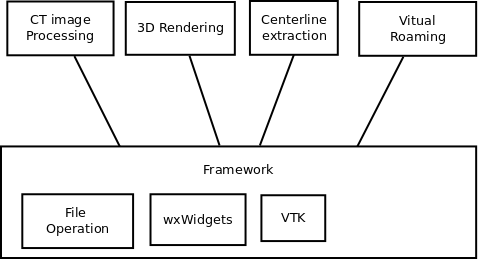
\includegraphics[width=350bp]{figure/structure.png}
    \caption{系统总体架构图}
    \label{structure}
\end{figure}

底层框架层:包含文件操作类,图形界面库wxWidgets和VTK库用来进行高效的渲染。上层应用类使用底层框架提供的功能,实现具体功能。下面分模块阐释:
\section{CT图像处理和3D重建模块}
在医学影像信息学的发展过程中,由于医疗设备生产厂商的不同,造成与各种设备有关的医学图像存储格式、传输方式千差万别,使得医学影像及其相关信息在不同系统、不同应用之间的交换受到严重阻碍。为规范医学影像及其相关信息的交换, DICOM(Digitalimaging and Communications in Medicine)标准就是在这样的背景下产生了。

由于VTK/ITK对DICOM格式支持有限,本系统主要使用GDCM库来实现对DICOM格式的CT图像的读取。读取CT图像后先进行滤波操作去除噪点,然后使用ITK的Connected Threshold算法对图像进行分割,通过良好的种子点和阈值选择,可以得到良好的分割效果,过程如图\ref{ct-process}。
\begin{figure}[h!]
    \centering
    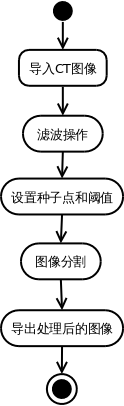
\includegraphics[width=100bp]{figure/ct_process.png}
    \caption{CT图像处理}
    \label{ct-process}
\end{figure}

处理完成的图像由于轮廓鲜明,使用VTK可以很方便地进行3D重建。同时,这里可以并且输出为网格数据,或者将分割到的图像层叠得到体数据。由于面渲染比体渲染快,渲染使用网格数据,而体数据给中心路径提取模块使用。

\section{中心路径提取模块}
中心路径的提取基于体数据,如果这个模块脱离系统使用,模块提供了一个简单的将网格数据体素化为体数据的Python脚本。

这个模块计算过程中,算法对体数据在3个坐标轴方向上切片,得到3个切片群。然后对每个切片通过增强快速行进法求2D骨架,这样就得到了3个骨架群,分别对应3个坐标轴方向。最后对这3个骨架群求交集,就可以得到最后的中心路径。
处理过程如图\ref{process_skel_extract}。
\begin{figure}[h!]
    \centering
    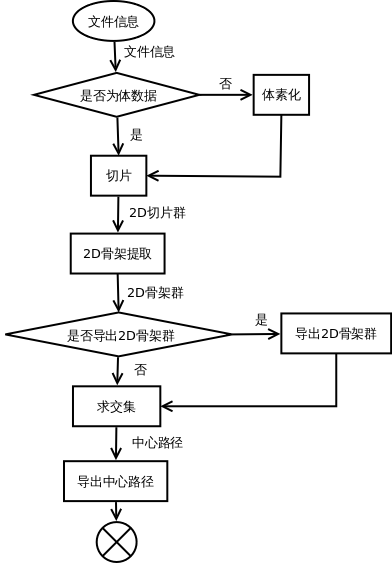
\includegraphics[width=300bp]{figure/process_skel_extract.png}
    \caption{中心路径提取过程}
    \label{process_skel_extract}
\end{figure}

\section{虚拟漫游模块}
虚拟漫游关键在于3D渲染,准确的路径和用户交互,上面两个模块已经得到了3D模型和准确的路径。这里使用wxWidgets图形库生成窗口,使用VTK渲染3D模型和处理用户的鼠标键盘输入,这样就可以实现虚拟漫游。

\section{本章小结}
本章从总体上把握了系统的架构。并对系统的上层应用层各个模块做了进一步设计,该部分可以为系统详细设计提供指导。
